%%%%%%%%%%%%%%%%%%%%%%%%%%%%%%%%%%%%%%%%%%%%%%%%%%%%%%%%%%%%%%%%%%%%%%%%%%%%%%%

\chapter{INTERVALFRAG}\label{ch:interval}

This section describes the IntervalFrag algorithm, and the proposed architecture needed to implement the enhancements to the Frag-Cubing's algorithm.

\section{Using Intervals in Inverted Indexes}\label{ch:interval:problem}

In chapter~\ref{ch:corr:cube:frag} the Frag-Cubing algorithm was explained, as per the original implementation by~\citeonline{liHighdimensionalOLAPMinimal2004}.
One of the key parts of the algorithm is the use of an inverted index to query directly into the attribute values and allow for the iceberg pruning of cells that fall below minimum support.
The algorithm depends on the intersection of TID lists to work, as that is how it can know what tuples have that specific value and where to find them to compute the relevant measures.
This part of the algorithm is mentioned by the original work as being done naively, and the original authors suggest some ways of compressing the index and speeding up the intersection of the lists, as this will be one of the most frequent operations that the algorithms needs to do to answer queries, and a speedup on this part would greatly enhance performance.

Furthermore, as most of the data is directly loaded into memory, using some form of compression on the inverted index would also reduce memory implementation requirements, and hopefully also query response times.
One of the strategies that they mention is by compressing the TID list into \textit{d-gaps}, in which each element is encoded by being the sum of the current element plus the previous element.
In general, for a list of numbers $\langle d_1, d_2 , \cdots, d_k \rangle$, the \textit{d-gap} list would be $\langle d_1 , d_2 - d_1 , \cdots, d_k - d_{k - 1} \rangle$.
The compression then would come from encoding the elements into a smaller number of bits, hopefully much less than the standard of 32 for an integer.
This approach takes advantage of the ordered nature of the TID list, as it is encoded from the tuples as they read and thus are naturally sorted non-zero positive integers.

This approach requires heavily changing the binary operations of the inverted index, however it is not the only one: since publication there are various different techniques to compress an inverted index, and they are an active branch of research.
More options, and a more complex implementation of the above method can be found into Elias-Fano encoding and the others mentioned in~\citeonline{pibiriTechniquesInvertedIndex2019}.
However, most of them require the use of dictionaries or heavy bit-encoding to achieve better results, which in general sacrifices the update operation.

One much simpler technique that has not been explored is the use of intervals instead of raw numbers in the TID list.
The inverted index structure is then kept, but each TID list now instead of containing the ordered numbers, contains an ordered list of intervals between each element.
For a list of numbers $\langle d_1, d_2 , \cdots, d_k \rangle$, the interval list would be $\langle [d_1, d_2] , [d_3, d_4], \cdots, [d_k, d_{k + 1}] \rangle$, where $d_k < d_{k+1}$, and the difference between the intervals cannot be smaller than one, thus $d_{k+1} - d_k \geq 1$.
Example: for the TID list $\langle 1, 3, 4, 5, 7 \rangle$, the Interval List would be $\langle [1, 1], [3, 5], [7, 7] \rangle$, where we can represent $3$ and $7$ that have no difference between their intervals as the singles $\langle [1], [3-5], [7] \rangle$.

This has implications only for the intersection of the lists, and is overall a much simpler implementation to execute.
By previous experience with the data, it was found that a great number of dimensions have attribute values that are repeated on long sequences of the same telemetry data points, and Frag-Cubing generates a long list of these repetitions for some dimensions.
This work then seeks to answer the question: \textbf{Can the use of the Interval algorithm instead of the raw list reduce memory requirements and query response times for long sequences of real world satellite telemetry data?}

Thus, in this chapter this implementation will be detailed, as well as an experiment to evaluate whether there is any advantage to using these intervals over the standard technique used by Frag-Cubing.

\section{Algorithm}\label{ch:interval:algo}

In practice, the algorithm cannot be implemented using two integers for each interval, as in the case where there is not a substantial interval (difference bigger than one) all elements will take the space of two integers when in Frag-Cubing they would take the place of only one integer.
This would lead to the worst case for the Interval algorithm to be double the memory of Frag-Cubing, but this can be worked around in practice by encoding the elements without an interval in the negative range of the integer, which isn't used in the TID list as each element indicates a unique identifier that is positive.

In case the identifier to be inserted would be close to zero, it is necessary to add one to each of the elements in the TID list as they are inserted into the IntervalIndex, as checking for a negative zero is not recommended and not guaranteed to work the same on every computer architecture \cite{ieeeIEEEStandardFloatingPoint2019}.
With this, the entire integer bit space is used, including the signal bit for the algorithm.
For the scope of this work, and since the experiment does not require the update of cells, only the insertion and intersection algorithms will be detailed.

Furthermore, it is necessary to define the concept of sequentiality, as it quantifies how much a list can be compressed by transforming it into a list of intervals.
A high sequentiality means that the data are repeated in long sequences, for example $\langle 1, 2, 3, 4, 5, 6, 7, 8, 9 \rangle$ can be compressed into the sequences $\langle [1, 9] \rangle$, being of high sequentiality.
However, the list $\langle 1, 3, 5, 6, 9\rangle$ would have a low sequentiality, as the resulting list interval would be only $\langle [1], [3], [5, 6], [9] \rangle$, and would consume exactly as much space as the raw list, with the conversion to an interval list being unfavorable.

\subsection{IntervalInsertion}\label{ch:interval:algo:insertion}

Insertions to the index can be done always by appending to the current list, as the TID are read in sequence and are naturally ordered positive integers.
Supposed that we're inserting an element $b$ to the list.
The insertion can be done by checking if the last element in the list is positive, if it is, then there is an interval and it is necessary to check the penultimate element in the list.
If the last element is negative $c$, then we can check if $c * -1 + 1 = b$, and if it is we flip the signal of the position $c$ and insert $b$ to the list as it is.
If the last element is not negative, then we check if the element $c$, is $c + 1 = b$ and update the position $c$ if it is true, else we flip the signal of $b$ and insert it at the end of the list.
Else none of these we can safely append $b$ to the end of the list after flipping the signal to negative, and thus this algorithm is implemented at $\Theta(1)$, shown in \autoref{algo:interval_insertion}.

\begin{algorithm}[!htb]
\SetAlgoLined
\KwResult{Element inserted into the list}
 $b$ element to be inserted\;
 $L$ the interval list to be inserted\;
 \If{$empty(L)$}{
   AppendList($L$, $b * - 1$)\;
   \KwRet\;
 }
 $c$ = LastElement($L$)\;
 \eIf{$c < 0$}{
   \If{$c * -1 + 1 = b$}{
     $L[c] = L[c] * - 1$ \tcp*{Update the last to be positive}
     AppendList($L$, $b$)\;
     \KwRet\;
   }
 }{
   \If{$b + 1 = c$}{
     $L[c] = b$ \tcp*{Update last element}
     \KwRet\;
   }
 }
 AppendList($L$, $b * - 1$) \tcp*{None of the previous cases, just append the element as a negative}
 \caption{IntervalInsertion}\label{algo:interval_insertion}
\end{algorithm}

\subsection{IntervalIntersection}\label{ch:interval:algo:intersection}

The problem of intersecting two sets of elements is a big one, and will not be fully explored by this work, however a simple exploration of some algorithms that was a byproduct of this work are available in Appendix~\ref{ap:a:problem}.
However, due to the change in how the index uses the TID list, it is necessary to adapt the Frag-Cubing set intersection algorithm to still calculate the intersection between two intervals, and so the IntervalIntersection algorithm is created.

In order to check if two intervals intersect: assuming two intervals $I_a = \langle a_l, a_r \rangle$ and $I_b = \langle b_l, b_r \rangle$, where $a_l$ is the smallest element in the interval, and $a_r$ the biggest element in the interval.
The output intersection can be defined as $I_o = \langle a_l, a_r \rangle$, and the intersection $I_o = I_a \bigcap I_b$ can be computed by computing the biggest element between $a_r$ and $b_r$ (function $max$) and the smallest element between $a_l$ and $b_l$ (function $min$), or \autoref{algo:intersect_interval}.

\begin{algorithm}[!htb]
\SetAlgoLined
\KwResult{The result intersection $I_o$, or $\emptyset$ in case there is no intersection}
 $I_a$ and $I_b$ two intervals\;
  \eIf{$b_l > a_r$ or $a_l > b_l$}{
    \KwRet $\emptyset$\;
  }{
  $o_l$ = $max( a_l, b_l )$\;
  $o_r$ = $min( a_r, b_r )$\;
  \KwRet $[o_l, o_r]$\;
  }
  \caption{IntersectTwoIntervals, adapted from \cite{26260}}\label{algo:intersect_interval}
\end{algorithm}

\autoref{fig:interval:sample} shows four examples of using this algorithm to select for intersections, including the empty case when there is no intersection.
For the list interval intersection, it can be naively implemented using the scalar merge strategy: two pointers walk by each interval, check if there is an intersection between then and, if there is, create a new element in the result list with the intersection between these two intervals.
The algorithm to perform this is shown below, and takes the same complexity of the parent algorithm of $\mathcal{O}(n + m)$, where $n$ and $m$ are the sizes of the interval lists being intersected.
This resulting algorithm is based on the implementations by \citeonline{liHighdimensionalOLAPMinimal2004} and \citeonline{silva:2015:abordagensParaCubo}, shown in \autoref{algo:intersect_interval_lists}.

\begin{figure}[!htb]
  \caption{IntervalIntersection example}\label{fig:interval:sample}
  \vspace{6mm}
  \begin{center}
    \resizebox{9cm}{!}{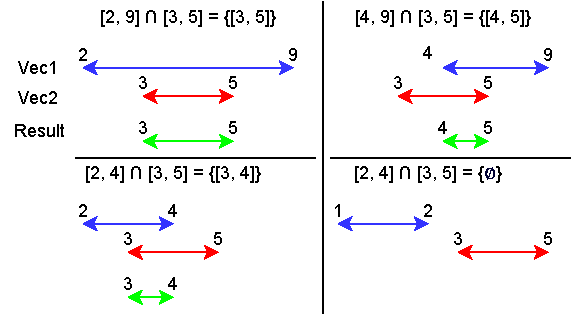
\includegraphics{Figuras/IntervalIntersection-Cases.pdf}}
  \end{center}
  \vspace{2mm}
  \legenda{IntervalIntersection example with four operations}
  \FONTE{Author}
\end{figure}

\begin{algorithm}[H]
\SetAlgoLined
\KwResult{The resulting list intersection between two interval lists, or $\emptyset$ if there is no intersection}
 $L_a$ and $L_b$ two input interval lists\;
 $L_c$ result list, with maximum size $min(length(L_a), length(L_b))$\;
 $a_i, b_i, c_i = 0$\;
 \While{$a_i < length(L_a)$ and $b_i < length(L_b)$}{
   $A[a_l, a_r]$ = interval($L_a[a_i$]) \tcp*{Gets the interval at this position}
   $B[b_l, b_r]$ = interval($L_b[a_i$])\;
  \If{$b_l \leq a_r$ and $a_l \leq b_r$}{
    IntervalInsertion($L_c$, IntersectTwoIntervals(A, B)) \tcp*{Insert into the result list the intersection between the elements}
    NextIntervalPosition($c_i$) \tcp*{Skips to the next available list space}
  }
  \eIf{$a_r \leq b_r$}{
   NextIntervalPosition($a_i$)\;
   }{
   NextIntervalPosition($b_i$)\;
  }
 }
 \KwRet{$L_c$}\;
 \caption{IntervalIntersection}\label{algo:intersect_interval_lists}
\end{algorithm}

\section{Results}\label{ch:interval:results}

\autoref{tab:interval_memory} and~\autoref{tab:interval_query} show the results of executing both algorithms to answer the queries defined in \autoref{ch:querypart:queries}, while using the cube structure defined as $C0$ in \autoref{ch:querypart:exp:method}, where all telemetries were used as a single file for each test, and then the query was executed, measuring the memory consumption in the first and query response time in the latter.

\begin{table}[!ht]
  \centering
  \caption{IntervalFrag x Frag-Cubing, memory consumption in KiB}\label{tab:interval_memory}
  \begin{tabular}{|c|c|c|c|c|c|c|c|}
    \hline
    & & \multicolumn{5}{c|}{\textbf{Tuples}} \\
    \hline
    \bfseries Algorithm & \bfseries Query & \bfseries $2\times10^6$ & \bfseries $4\times10^6$ & \bfseries $6\times10^6$ & \bfseries $8\times10^6$ & \bfseries $1\times10^7$\\
    \hline
    \multirow{5}{*}{Frag-Cubing} & Q1 &
    1.908.708 & 3.674.784 & 5.447.864 & 6.953.424 & 8.557.348
    \\\cline{2-7} & Q2 &
    1.842.396 & 3.294.628 & 4.727.816 & 5.877.016 & 6.760.080
    \\\cline{2-7} & Q3 &
    1.448.280 & 2.836.592 & 4.236.496 & 5.362.128 & 6.502.628
    \\\cline{2-7} & Q4 &
    1.444.816 & 2.836.696 & 4.236.404 & 5.372.104 & 6.520.176
    \\\cline{2-7} & Q5 &
    1.607.456 & 3.024.996 & 4.445.800 & 5.591.052 & 6.650.456
    \\\hline
    \multirow{5}{*}{IntervalFrag} & Q1 &
    504.428 & 845.804 & 1.196.504 & 1.455.472 & 1.651.552
    \\\cline{2-7}
    & Q2 &
    801.864 & 1.207.760 & 1.560.652 & 1.752.292 & 2.062.560
    \\\cline{2-7} & Q3 &
    388.652 & 707.588 & 1.030.392 & 1.237.324 & 1.415.472
    \\\cline{2-7}
    & Q4 &
    370.624 & 690.456 & 1.003.236 & 1.237.292 & 1.415.456
    \\\cline{2-7}
    & Q5 &
    540.788 & 895.272 & 1.232.520 & 1.412.280 & 1.604.288
    \\\hline
  \end{tabular}
\end{table}

\begin{table}[!ht]
  \centering
  \caption{IntervalFrag x Frag-Cubing, query response times in ms}\label{tab:interval_query}
  \begin{tabular}{|c|c|c|c|c|c|c|c|}
    \hline
    & & \multicolumn{5}{c|}{\textbf{Tuples}} \\
    \hline
    \bfseries Algorithm & \bfseries Query & \bfseries $2\times10^6$ & \bfseries $4\times10^6$ & \bfseries $6\times10^6$ & \bfseries $8\times10^6$ & \bfseries $1\times10^7$\\
    \hline
    \multirow{5}{*}{Frag-Cubing} & Q1 &
    5.4691 & 188.634 & 310.455 & 421.409 & 523.772
    \\\cline{2-7} & Q2 &
    47.391 & 108.405 & 170.515 & 258.585 & 281.877
    \\\cline{2-7} & Q3 &
    1.557 & 3.089 & 4.637 & 6.497 & 7.597
    \\\cline{2-7} & Q4 &
    399 & 817 & 1.193 & 1.573 & 1.990
    \\\cline{2-7} & Q5 &
    7.138 & 21.668 & 33.483 & 49.590 & 59.428
    \\\hline
    \multirow{5}{*}{IntervalFrag} & Q1 &
    1.946 & 4.712 & 6.981 & 9.198 & 11.508
    \\\cline{2-7}
    & Q2 &
    158.050 & 333.838 & 554.111 & 772.125 & 934.793
    \\\cline{2-7} & Q3 &
    3.570 & 7.064 & 10.655 & 14.812 & 17.714
    \\\cline{2-7}
    & Q4 &
    995 & 2.011 & 2.952 & 3.860 & 4.916
    \\\cline{2-7}
    & Q5 &
    4.871 & 11.837 & 18.477 & 26.176 & 32.649
    \\\hline
  \end{tabular}
\end{table}

In order to make the comparisons easier to understand, let's focus on only queries $Q1$ and $Q2$, that were the highest number of dimensions and the highest number of cardinalities respectively.
\autoref{fig:interval:q1-2} shows those results, and it is clear that the memory usage is always much lower under IntervalFrag.
$Q1$ has four dimensions with low cardinality and high sequentiality, and these are quickly answered by IntervalFrag, while Frag-Cubing takes a long time to answer the queries that involve those dimensions.

However, in the case of $Q2$ where all dimensions have both cardinality and low sequentiality, IntervalFrag takes 331\% longer to answer the query on the worst case, being the biggest drawback of this algorithm.
This is due to the inherently slower set intersection algorithm used by IntervalFrag, that needs to execute more comparisons than Frag-Cubing, even when the algorithms have the same complexity and are similar.

\begin{figure}[H]
  \caption{IntervalFrag for Q1 and Q2}\label{fig:interval:q1-2}
  \vspace{6mm}
  \begin{center}
    \resizebox{13cm}{!}{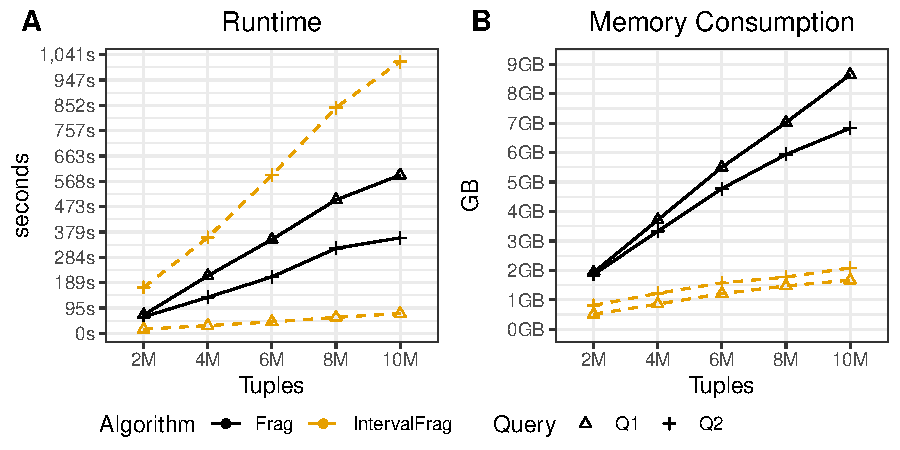
\includegraphics{Figuras/q1q2-1.pdf}}
  \end{center}
  \vspace{2mm}
  \legenda{
    (\textbf{A}) Query response times of IntervalFrag and Frag-Cubing for queries $Q1$ and $Q2$ under the cube $C0$
    (\textbf{B}) Memory consumption of IntervalFrag and Frag-Cubing for queries $Q1$ and $Q2$ under the cube $C0$.
}
  \FONTE{Author}
\end{figure}

In the case of queries $Q3$, $Q4$ and $Q5$, IntervalFrag is slower to answer queries $Q3$ and $Q4$, both that have a high cardinality and low sequentiality, but takes only about 53\% of the time to answer $Q5$, that also has a high cardinality but presents a high sequentiality.
\autoref{fig:interval:q3-4} shows those results for $Q3$ and $Q4$, \autoref{fig:interval:q5} for $Q5$, and it is also clear that the memory usage is much lower with IntervalFrag than with Frag-Cubing.

\begin{figure}[H]
  \caption{IntervalFrag for Q3 and Q4}\label{fig:interval:q3-4}
  \vspace{6mm}
  \begin{center}
    \resizebox{13cm}{!}{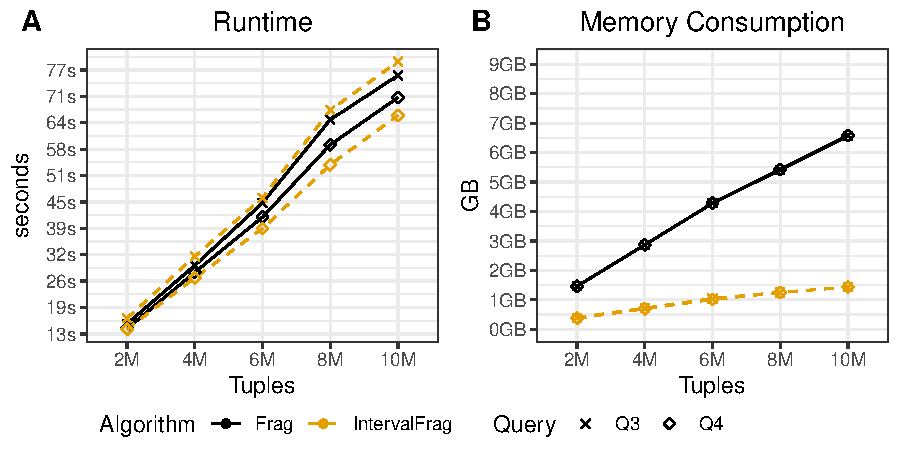
\includegraphics{Figuras/q3q4-1.pdf}}
  \end{center}
  \vspace{2mm}
  \legenda{
    (\textbf{A}) Query response times of IntervalFrag and Frag-Cubing for queries $Q3$ and $Q4$ under the cube $C0$
    (\textbf{B}) Memory consumption of IntervalFrag and Frag-Cubing for queries $Q3$ and $Q4$ under the cube $C0$.
}
  \FONTE{Author}
\end{figure}

\begin{figure}[H]
  \caption{IntervalFrag for Q5}\label{fig:interval:q5}
  \vspace{6mm}
  \begin{center}
    \resizebox{13cm}{!}{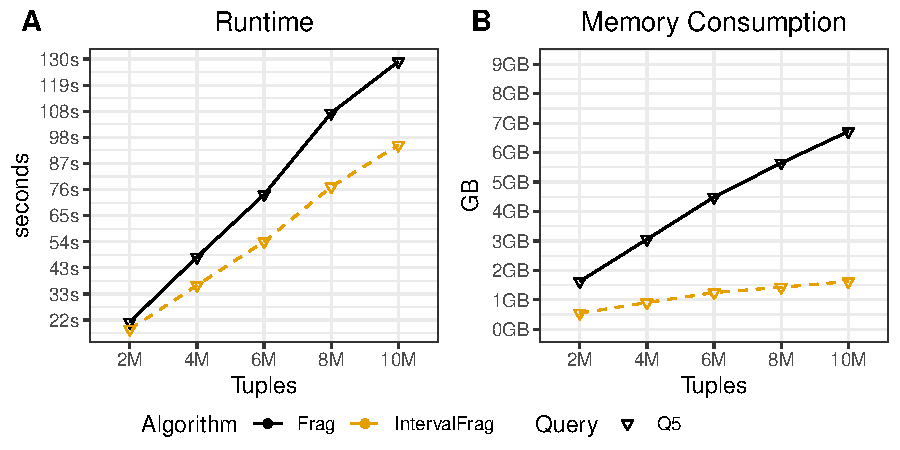
\includegraphics{Figuras/q5-1.pdf}}
  \end{center}
  \vspace{2mm}
  \legenda{
    (\textbf{A}) Query response times of IntervalFrag and Frag-Cubing for queries $Q5$ under the cube $C0$
    (\textbf{B}) Memory consumption of IntervalFrag and Frag-Cubing for queries $Q5$ under the cube $C0$.
}
  \FONTE{Author}
\end{figure}

Additionally, we need to compare the time necessary to create the cube under each of the algorithms, here called Time to Cube.
If one algorithm takes too long to transverse the cube structure and execute the minimum support pruning this would need to be counted against it, however as~\autoref{fig:interval:timetocube} shows, the difference between IntervalFrag and Frag-Cubing is not that big, with IntervalFrag being on average 10\% slower than Frag-Cubing.
This however is just a simple comparison, as in that step each subcube of the fragments would be computed and for these tests that use $\mathcal{F} = 1$ they are almost exactly the same computation, needing higher fragment sizes to appreciate the difference.
However, since this computation would involve list intersections at higher fragment sizes, the speed of the intersection algorithm would heavily influence this computation, being more comparable to the query response times compared above.

\begin{figure}[H]
  \caption{Comparison: Time to Cube}\label{fig:interval:timetocube}
  \vspace{6mm}
  \begin{center}
    \resizebox{13cm}{!}{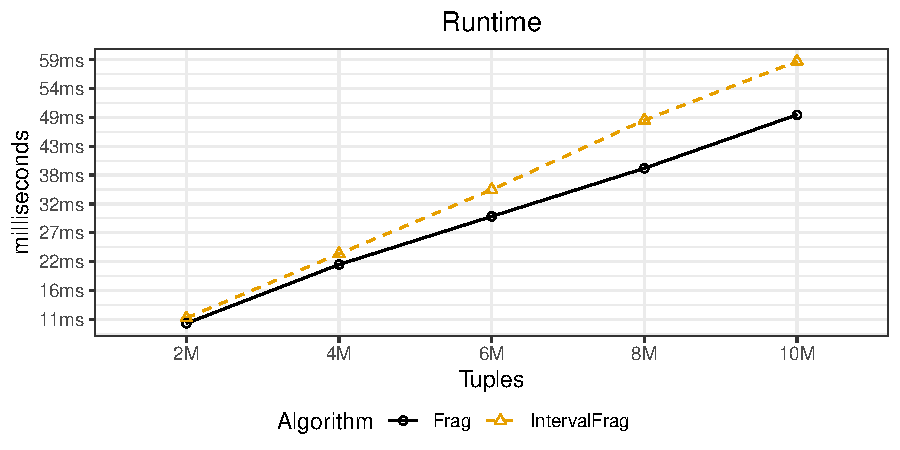
\includegraphics{Figuras/timetocube-1.pdf}}
  \end{center}
  \vspace{2mm}
  \legenda{Time necessary to compute the cube after the data is read into memory.}
  \FONTE{Author}
\end{figure}

Another important metric is the baseline memory used before queries can be performed on the data.
\autoref{fig:interval:baseline} shows these values for the files used in this experiment, and IntervalFrag consumes on average 22\% of the memory that Frag-Cubing needs.
This is important as it allows IntervalFrag to be implemented while requiring much less computational resources.

\begin{figure}[H]
  \caption{Comparison: Baseline memory}\label{fig:interval:baseline}
  \vspace{6mm}
  \begin{center}
    \resizebox{13cm}{!}{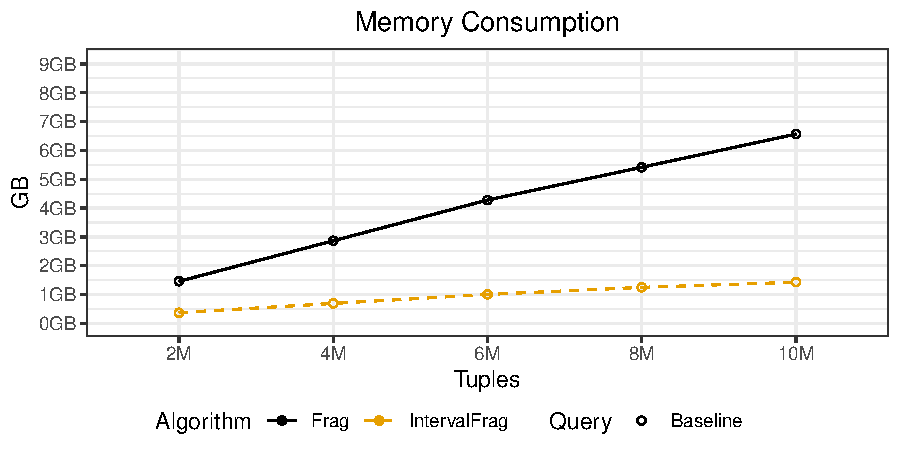
\includegraphics{Figuras/baseline-1.pdf}}
  \end{center}
  \vspace{2mm}
  \legenda{Memory used by the baseline cube, when it can start to answer queries}
  \FONTE{Author}
\end{figure}

\section{Summary}\label{ch:interval:summary}

FragInterval was up to 3 times slower to answer queries on dimensions with low sequentiality and high cardinality, but was faster to answer queries on dimensions with high sequentiality.
On all queries FragInterval used only between 20\% and 24\% of the memory that Frag-Cubing used, being the biggest improvement that IntervalFrag brings.
Furthermore, FragInterval also needed only on average 22\% of the memory that Frag-Cubing used to compute the baseline cube, before the queries can be answered, while being only 10\% slower to compute.

Thus, FragInterval shows to be preferred on environments with low available RAM, as long as the slower queries with higher cardinalities are acceptable.
FragInterval achieves the objective of answering the queries with much less memory, however fails at having comparable response times than Frag-Cubing on high dimensionality queries.
This slowness is due to the set intersection algorithm in IntervalFrag having to execute more comparisons in practice than Frag-Cubing's, and thus being slower when the sets have the same size and the data has low sequentiality to favor IntervalFrag's algorithm.

